\label{ssub:实验心得}
本次作业共用时约50小时. 其中20小时45分钟在C++程序代码编写和测试上,
17小时39分钟在Rust程序代码编写和测试上, 3小时21分钟在makefile
的编写和修改上, 7小时18分钟在tex实验报告的编写上.\par
% \begin{figure}[ht!]
% 	\begin{center}
% 		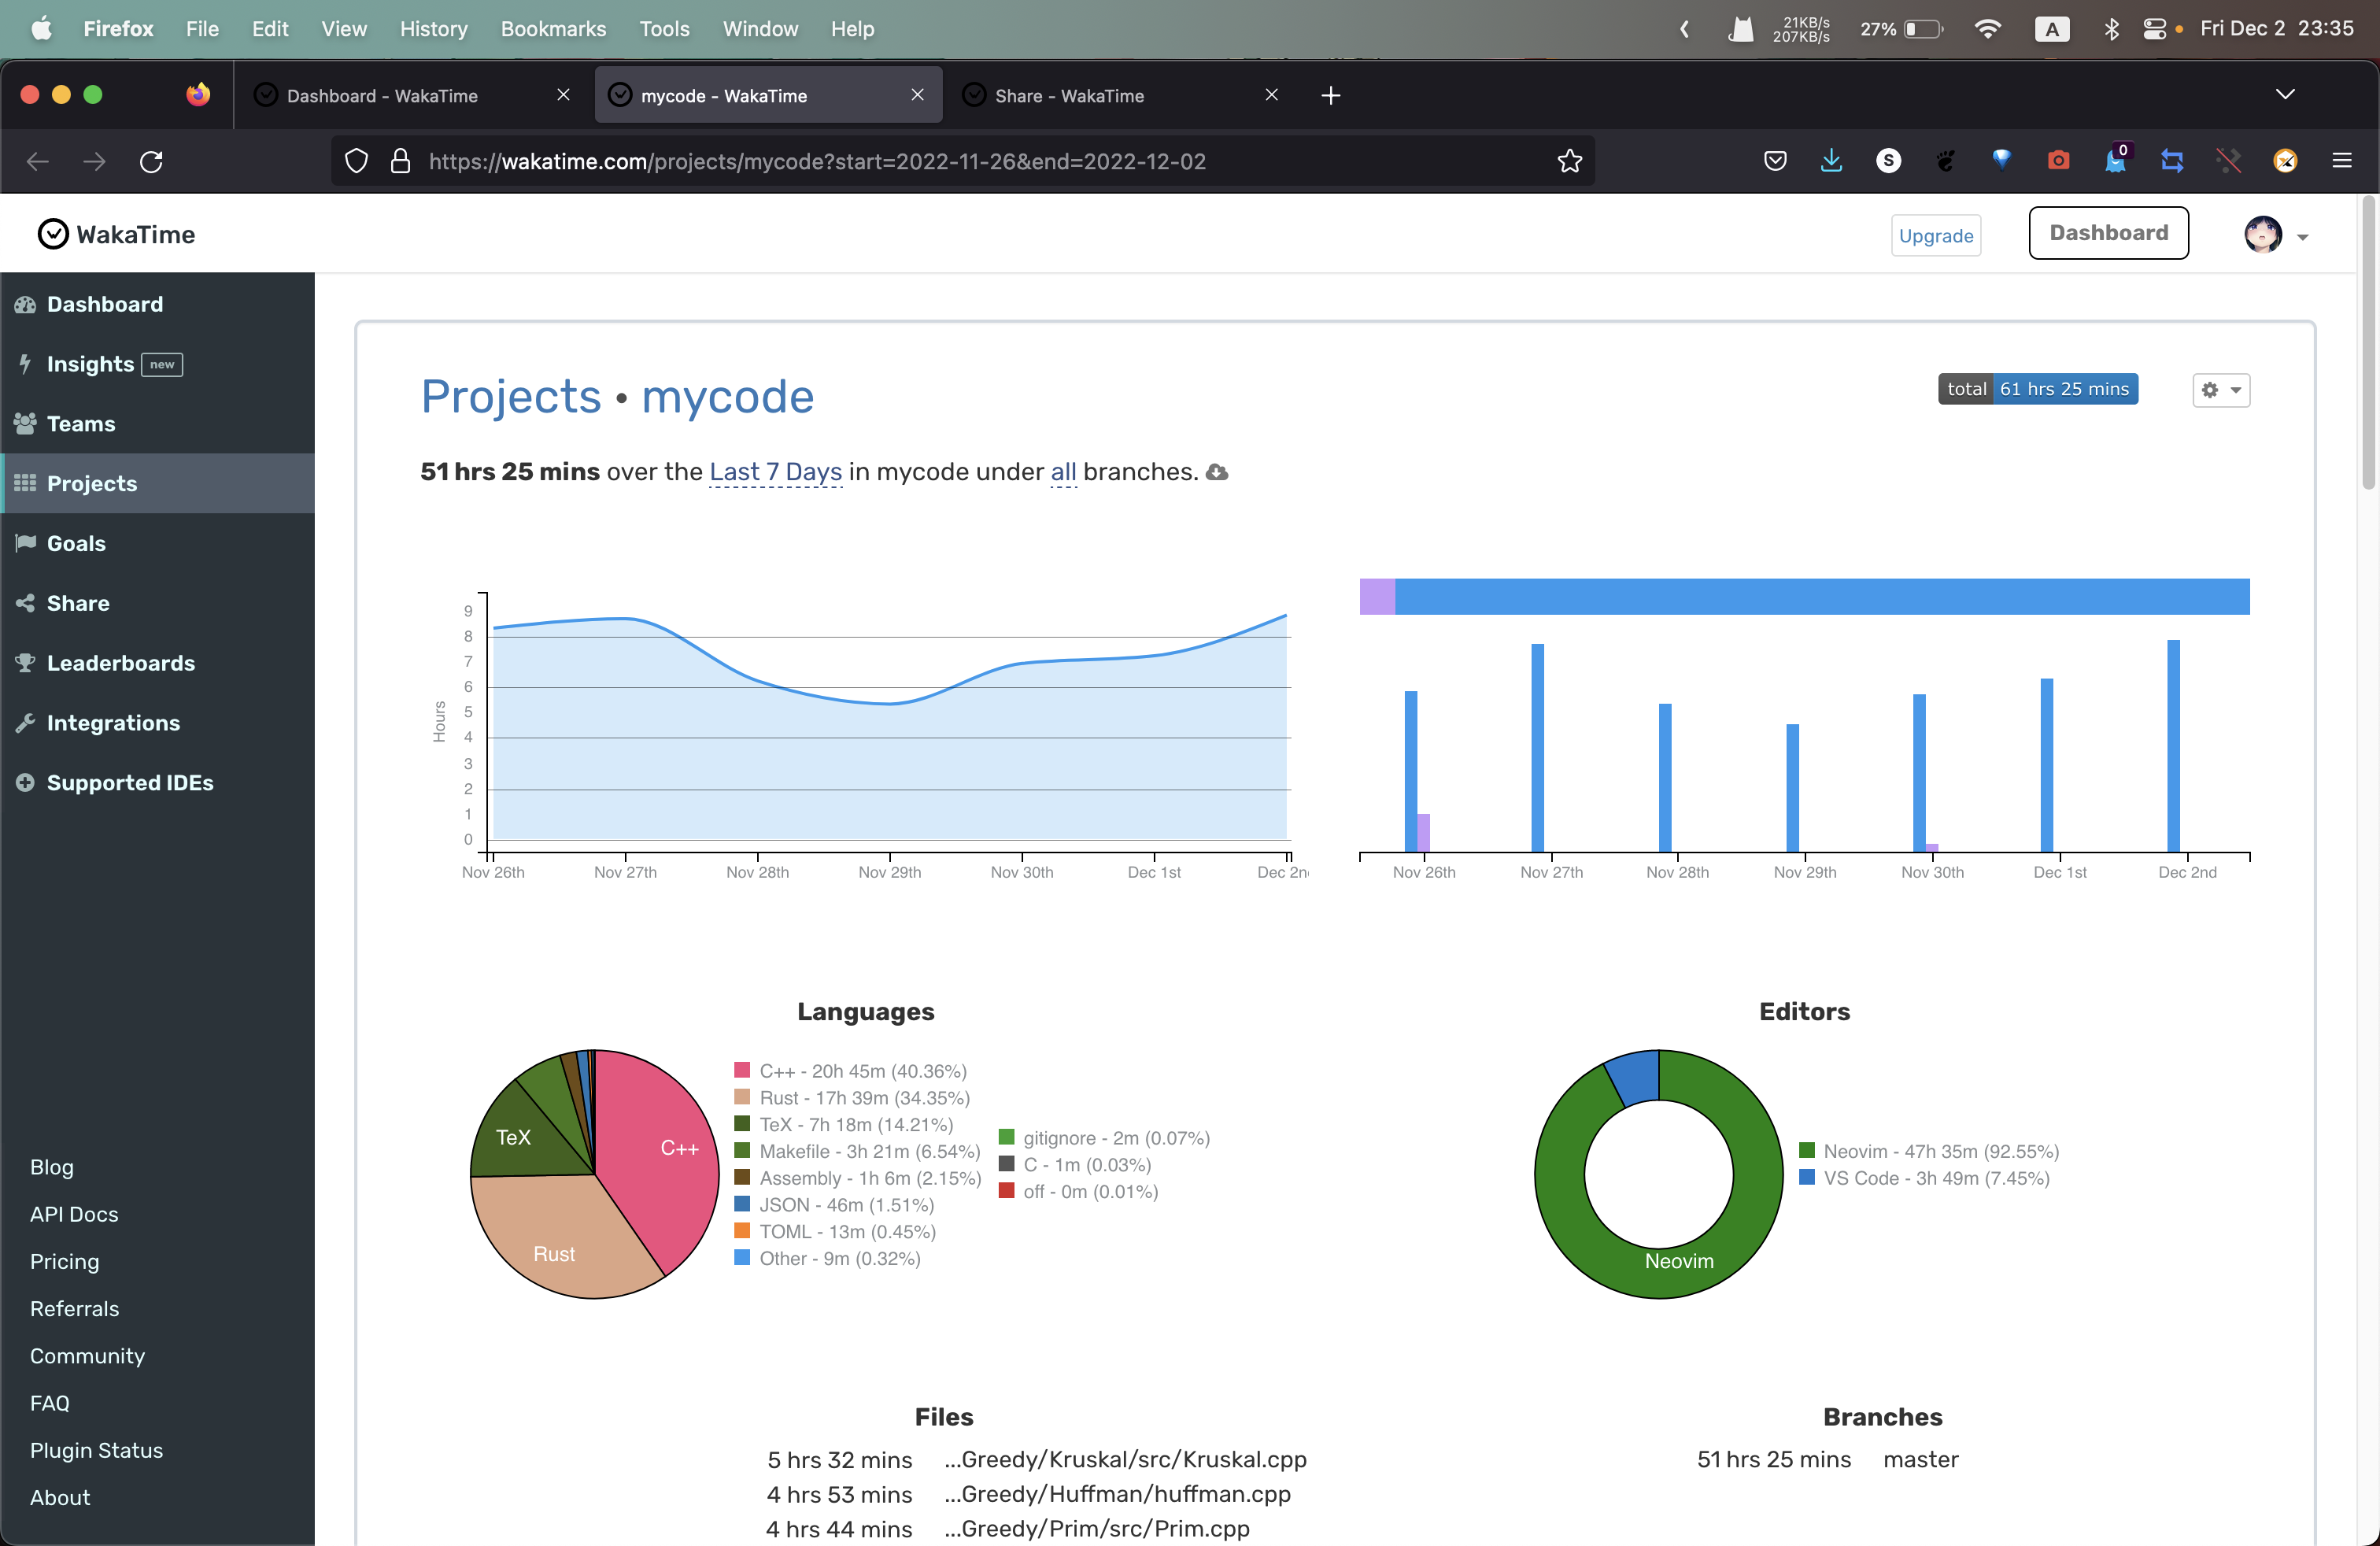
\includegraphics[width=0.95\textwidth]{time-statistics.png}
% 	\end{center}
% 	\caption{编写时间统计}
% 	\label{fig:screenTime}
% \end{figure}
% 统计链接: \href{https://wakatime.com/@micuks/projects/uemupyroug?start=2022-11-26&end=2022-12-02}{编码时间统计}

通过这次实验, 我动手实现了Huffman, Dijkstra, Prim,
Kruskal算法及其用到的MinHeap和Disjoint-set union算法. 动手实践了
各算法的时间复杂度和空间复杂度分析. 此外, 为了综合评价各算法的
正确性, 以及衡量各算法的性能, 还动手实现了数据生成器, 用来
方便的生成指定数量的均匀分布在给定范围的随机排序的数据作为排序程序的输入.\par

借助这次实验, 我还对Rust语言进行了学习, 并与C++进行了比较.
因为Rust语言还比较生疏, 所以Rust编写程序花费的时间要比C++要长一些.
但是Debug的时间却短得多, 说明Rust严格的编译检查除了能确保内存严格安全之外,
实际上反而能帮助程序员节省时间在内存相关的debug上.\par

在构建和管理项目的工具方面, 使用了make工具, 方便的实现了
对程序的构建和测试; 此外, 对于文档, 也使用了make工具作为管理,
很大程度上方便了实验报告修改后的再次编译. 在实验报告编写方面,
练习了latex的使用, 对latex语法和使用更加熟悉.\par

但是, 由于时间有限, 没有实现更多的优化内容, 比如Fibonacci Heap代替BinaryHeap等.\par

总的来说, 这次实验在动态规划算法之内及之外都学到了许多知识, 收获颇丰.
% subsection 实验心得 (end)
